
%\documentclass[conference]{IEEEtran}
\documentclass{sig-alternate}

\usepackage{cite}
\usepackage{color}
\usepackage{courier}
\usepackage{url}
\usepackage{tikz}

\usepackage{balance} % Add this back in. Probably needed during camera ready.
\usepackage[numbers]{natbib} % Used to fix formatting issue.
\usepackage{pgfplots}

%%

%\usepackage{graphicx}% http://ctan.org/pkg/graphicx

%\usepackage{listings}
%\usepackage{pxfonts}
%\usepackage{times}
%\usepackage{xspace}
%\usepackage{booktabs}
%\usepackage{fancybox}

%\usepackage{multirow}
%\usepackage{array}
%\usepackage{tabularx}
%\usepackage{url}
%\urlstyle{same}
%\usepackage{xcolor}


\usepackage{caption}
\usetikzlibrary{shapes,arrows}
\usetikzlibrary{patterns}
\usepackage[numbers]{natbib} % Used to fix formatting issue.
\usepackage{soul} % Needed for wrapping of highlighted text

% Define bar chart colors
%
\definecolor{bblue}{HTML}{4F81BD}
\definecolor{rred}{HTML}{C0504D}
\definecolor{ggreen}{HTML}{9BBB59}
\definecolor{ggrey}{HTML}{707070}
%\definecolor{ppurple}{HTML}{9F4C7C}


% Define flow chart styles
\tikzstyle{decision} = [diamond, draw, fill=blue!20,
    text width=15em, text badly centered, node distance=3cm, inner sep=0pt]
\tikzstyle{block} = [rectangle, draw, fill=blue!20,
    text width=15em, text centered, rounded corners, minimum height=4em]
\tikzstyle{line} = [draw, -latex']

\usetikzlibrary{shapes,arrows, positioning} % Needed for analysis diagram

\newcommand{\todo}[1]{\textcolor{cyan}{\textbf{[#1]}}}
%\newcommand{\xxx}[1]{\textcolor{green}{{\it [xxx says: #1]}}}
\newcommand{\dan}[1]{\textcolor{blue}{{\it [Dan says: #1]}}}
%\newcommand{\andy}[1]{\textcolor{blue}{{\it [Andy says: #1]}}}
%\newcommand{\sam}[1]{\textcolor{blue}{{\it [Sam says: #1]}}}



\begin{document}

% Update this title?
\title{XWhy Permission-Gaps Occur in Android Applications, their Effects, and How they can be Prevented.X}

\numberofauthors{1}

\author{
%
% 1st. author
\alignauthor
XXXXXXXXXXXXXXXXXXXXXXX\\ 	
	\affaddr{Software Engineering Department}\\
       \affaddr{Rochester Institute of Technology}\\
       \affaddr{1 Lomb Memorial Drive}\\
       \affaddr{Rochester, NY, USA} \\
       \email{\{dxkvse, xxx\}@rit.edu}
}
\maketitle



\begin{abstract}
Abstract

% Write up the abstract to give us an idea of what we are going to be working on


% Main focal point of paper
%   Why do over privs occur
%   When do they occur
%   How can they be prevented
%   How do overprivs and Androrisk affect security
%Secondary
%   Show lifecycle of security over several Android apps



\end{abstract}



\section{Introduction}






\section{Research Questions}
\label{sec: researchquestions}


\textbf{RQX:}~\emph{What are the most pervasive overprivileges?}\\
% Describe why they occurred
Blah


\textbf{RQX:}~\emph{What is the variation of risks across genres?}\\
Blah


\textbf{RQX:}~\emph{How does code quality ?}\\
Blah


\textbf{RQX:}~\emph{What causes apps to be under prived? ?}\\
Blah
%   Are certain kits/uses the cause of apps being over prived? - For example, "android.webkit.WebView.<init>: [android.permission.INTERNET]" - leads an app to be over prived?
%       Is this a problem with the tool?


\textbf{RQX:}~\emph{Why do over privs occur and what can be done to prevent them?}\\
Blah
%%%% Analyze

%%  When are they introduced in the development cycle
%%  Do the same methods have overprivs? - Could this just be related to the selected tool. Maybe the tool messes up in the same areas?
%%  



\textbf{RQX:}~\emph{How does code quality, and the vulnerability of apps compare over time ?}\\
%%% Look at the lifecycle of apps
Blah


\textbf{RQX:}~\emph{Do developers ever remove permissions?}\\
%%% Look at the lifecycle of apps
Look at commit histories and app histories to see if developers ever add permissions to apps and then remove them.


%% Look at SQL to see the lifecycle of overprivs
%%  Initial results indicate that the overpriv rate only slightly increases


%% Look at Commit histories of apps to see the permissions in each commit





\textbf{RQX:}~\emph{What functionality additions cause over privs?}\\
%   Does stowaway say what caused the over privs?
%   Is there
%   Which permissions are most over prived?


% How many version/app updates actually deal with permissions? Do most just change small parts of functionality?
%   This may have been previously addressed. Mei's? work?



% Are there newer tools than stowaway?



% We collected Darwin to provide a larger result set
% Identical reverse engineering and analysis process was used on both
% Drive home that the same reverse engineering process has been used in other papers and is sound. Do not let people question what we are doing.



%% Look and see when permissions are added in general
%       Doesn't have to be an overpriv



% Do over privs lead to more overprivs?
%   If an app has 1 overpriv, is it more likely to be over prived?


%% Write a bash script to help with this?


% Commit keywords with an overpriv?
%   Bug fix
%   New commiter?



\label{sec: androidapplications}
\section{Android Applications}
%% External file so it can be easily included/excluded
%

The Android operating system is the most popular mobile platform in the world with apps being available on numerous types of devices from a variety of manufacturers~\cite{androidpopularity_url}. This flexibly has allowed the Android operating system to flourish, but results in many different hardware platforms and OS versions for app developers to support.

\subsection{Android Application Structure}

The Android application stack is comprised of four primary layers. The top layer is the Android application layer, which is followed by the the three application framework layers. The Android Software Development Kit (SDK) allows developers to create Android applications using the Java programming language. Isolation between Android applications is enforced through the use of the Android sandbox~\cite{androidsecuritytips_url}, which typically prevents applications from intruding upon one another.

\emph{Intents} are a communication mechanism to exchange information between the components (\emph{Activities}) of an Android application, and are reported to the user upon installation and use. Inter Process Communication (IPC) is the composition mechanism performed using Intents which is used to invoke another application component. Attacks that exploit Intents for malicious reasons include ~\emph{permission collusion},~\emph{confused deputy}, and~\emph{intent spoofing}~\cite{Chin:2011:AIC:1999995.2000018,grace2012systematic, Marforio:2012:ACC:2420950.2420958, 6641043}.

Android applications are packaged in APK files, which are compressed application files which includes the application's binaries and package metadata. Table~\ref{Table:apkcontents} shows the breakdown of a typical APK file.

%% Much of this able came from : ~\cite{Lee_2013}


\begin{table}[ht]% Try here, and then top
\begin{center}
\caption{APK Contents}
\label{Table:apkcontents}
  \begin{tabular}{| l | l | } \hline

    \bfseries File & \bfseries Description \\ \hline
    AndroidManifest.xml & Permissions \& app information \\ \hline
    Classes.dex & Binary Execution File \\ \hline
    /res & Directory of resource files \\ \hline
    /lib & Directory of compiled code \\ \hline
    /META-INF & Application Certification \\ \hline
    resources.arsc & Compiled resource file \\ \hline
  \end{tabular}
  \end{center}
\end{table}


Android applications are available from a variety of different locations including AppksAPK\footnote{http://www.appsapk.com/}, F-Droid\footnote{https://f-droid.org/}, and the GooglePlay store\footnote{https://play.google.com/store}. These stores differ from the iOS app store, which forces all non-jailbroken devices to access applications through an Apple controlled store. GooglePlay provides verification of uploaded applications using a service called Bouncer which scans applications for malware~\cite{bouncer_url1}. In spite of these efforts, malicious apps are sometimes found on the GooglePlay store~\cite{Zhou:2012:DAM:2310656.2310710}. GooglePlay separates apps into~\emph{Genres} based on their realm of functionality, some of which are Action, Business, Entertainment, Productivity, and Tools. The~\emph{AndroidManifest.xml} file contains permissions and application information as defined by the developer.

\subsection{Android Permission Structure}
Android developers operate under a permission-based system where apps must be granted access to various areas of functionality before they may be used. If an app attempts to perform an operation which it does not have permission, a~\emph{SecurityException} is thrown. When an Android app is created, developers must explicitly declare in advance which permissions the application will require~\cite{Felt:2011:APD:2046707.2046779}, such as the ability to write to the calendar, send SMS messages, or access the GPS.

When installing the application, the user is asked to accept or reject these requested permissions. Once installed, the developer cannot remotely modify the permissions without releasing a new version of the application for installation~\cite{shaerpour2013trends}, prompting the user if new permissions are required. These security settings are stored in the AndroidManifest.xml file and include a wide range of permissions, some of which are~\emph{INTERNET},~\emph{READ\_CONTACTS}, and~\emph{WRITE\_SETTINGS}. Unfortunately, developers often request more permissions than they actually need, as there is no built in verification system to ensure that they are only requesting the permissions their application actually uses~\cite{Felt:2011:APD:2046707.2046779}.

A basic principle of software security is the~\emph{principle of least privilege}, or the granting of the minimum number of privileges that an application needs to properly function~\cite{saltzer1975protection}. Granting more privileges than the application needs creates security problems since vulnerabilities in other applications, or malware, could use these extra permissions for malicious reasons. Additionally, this limits potential issues due to non-malicious developer errors. Unfortunately, due to the lack of granularity of the permission spectrum used by Android, the developer must often grant more permissions to their application than it actually requires. For example, an application that needs to send information to one site on the internet will need to be given full permissions to the internet, meaning that it may communicate with with all websites~\cite{jeon2011dr}.

In this study, we use the term \emph{overprivilege} to describe a permission setting that grants more than what a developer needs for the task. Likewise, an \emph{underprivilege} is a setting for which the app could fail because it was not given the proper permissions. Overprivileges are considered security risks, underprivileges are considered quality risks.





blah

\label{sec: appcollection}
\section{App Collection \& Static Analysis}
%% External file so it can be easily included/excluded
%


\todo{update and talk about how we collceted Data for F-droid}
We analyzed 30,020 Android application files over a period of 3 months using a variety of different tools. The results of this analysis have been stored in a publicly accessible database located on our project website\footnote{http://darwin.rit.edu}. Our methodology is as follows:

\begin{enumerate}
  \item Collect APK files
  \item Reverse-engineer binaries
  \item Execute static analysis tools
  \item Complete evaluation (see Section~\ref{sec: evaluation})
\end{enumerate}

We created the~\emph{Darwin} tool that downloads Android Application (.apk) files and invokes various static analysis tools against these files.

\label{sec: collection}
\subsection{Step 1: Collect APK files}


Android APK files were pulled from GooglePlay with a custom-built collector, which used~\emph{Scrapy}~\footnote{http://scrapy.org} as a foundation. We chose to pull from GooglePlay since it is the most popular source of Android applications~\cite{listofstores_URL} and was able to provide various application information such as the developer, version, genre, user rating, and number of downloads. To limit the impact of seldom-downloaded applications, we divided of our results into two groups: applications with at least 10,000 downloads, and those with less than 10,000 downloads. Of the 30,020 applications downloaded, 12,215 had at lt least 10,000 downloads, while 17,805 had fewer.

 %To limit the impact of seldom-downloaded applications, we only included applications with at least 10,000 downloads in our results. Of the 30,020 applications downloaded, 12,215 had at lt least 10,000 downloads, while 17,805 had fewer. In our presented results, unless otherwise noted the data set we will be referencing is the one comprising applications with at least 10,000 downloads. \dan{I added above...State why?}

\subsection{Step 2: Reverse-engineer binaries}
\label{sec: decompliation}
\todo{drive home that we are using a simlar process to what was done before. Show that we are using an estatblished, quality practice/}
Some of our static analysis tools require source code instead of binary code, so we followed a reverse engineering process similar to that as proposed by previous research~\cite{Lee_2013,6687155}. For many of our static analysis tools, the downloaded APK files had to be decompiled to .java files. The first step was to unzip the .apk file using a simple unix command, which creates the files shown in Table~\ref{Table:apkcontents}. Next, we used two open source tools to complete the reverse engineering process. These were:

\begin{itemize}
  \item \textbf{dex2jar~\cite{dex2jar_key}:} Convert the .dex file into a .jar file. A java jar command is then used to convert this to .class files.
  \item \textbf{jd-cmd~\cite{jdcmd_key}:} A command line decompiler that converts .class files to .java.
\end{itemize}

Additionally, we recorded the number of extracted class and java files. The de-compilation process is shown in Figure~\ref{fig:extractionprocess}.



% ~\cite{Lee_2013} %% This diagram is largely copied from here

% Define block styles
\tikzstyle{line} = [draw, -latex']
\tikzstyle{cloud} = [draw, ellipse,fill=white!20, node distance=2.2cm,
    minimum height=2em]

	\begin{figure}[h]
	\begin{center}
\label{fig:extractionprocess}
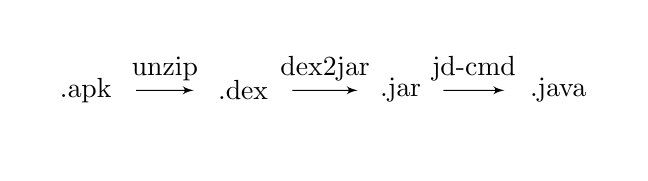
\begin{tikzpicture}[node distance = 2cm, auto]
    % Place nodes
     \node [cloud] (init) {.apk};
     \node [cloud, right of=init] (dex) {.dex};
     \node [cloud, right of=dex] (jar) {.jar};
     \node [cloud, right of=jar] (java) {.java};

     \path [line] (init) -- node {unzip}(dex);
     \path [line] (dex) -- node {dex2jar}(jar);
     \path [line] (jar) -- node {jd-cmd}(java);

\end{tikzpicture}
\caption{APK Extraction Process}
\end{center}
\end{figure}


\subsection{Step 3. Execute static analysis tools}
\label{sec: analysis}

The next phase was to analyze the extracted source code for a variety of metrics, including potential security risks, permissions issues, potential non-security defects, and misuse of coding standards. We also collected information about software clones, which are functionally equivalent portions of an application that may differ syntactically. A sign of poorly written software, clones may be detrimental to an application in a variety of ways, including increased maintenance costs and inconsistent bug fixes~\cite{Roy:2009:CEC:1530898.1531101}. We used the following tools for our analysis:

 \textbf{Stowaway\cite{Felt:2011:APD:2046707.2046779}:} Reports the overprivileges and underpriviledges of an application, which we recorded. Slight modifications were made to the existing version of Stowaway to accommodate our process and current Android applications with updated permissions. Permlyzer~\cite{6698893}, a more modern permission detection tool, was not used since its authors have not made it available for download.

 \textbf{AndroRisk\cite{androguard_url}:} A component of the Androguard reverse engineering tool which reports the risk indicator of an application for potential malware. We recorded the reported risk level for each APK file.

 \textbf{CheckStyle\cite{checkstyle_key}:} A development tool to measure how well developers adhere to coding standards such as annotation usage, size violations, and empty block checks. We recorded the total number of violations of these standards. Default application settings were used for our analysis.

 \textbf{Jlint\cite{jlint_key}:} Examines java code to find bugs, inconsistencies, and synchronization problems by conducting a data flow analysis and building lock graphs. We recorded the total number of discovered bugs. This tool was selected over FindBugs~\cite{findbugs_key} since it was able to analyze the applications much faster, while still providing accurate results~\cite{rutar2004comparison}.

 \textbf{Simcad\cite{6613857}:} A powerful software clone detection tool which we used to record the number of clones discovered for each target application.

 \textbf{APKParser\cite{apkparser_link}:} A tool designed to read various information from Android APK files including the version, intents, and permissions. We used the output from this tool to determine the application version, minimum SDK, and target SDK.

We also recorded other metrics about each application including total lines of code, number of java files, application version, target SDK, and minimum SDK.

% DK - Not sure if I should mention this part
%Whenever we were forced to slightly alter an existing application, we ensured its quality by testing it against \todo{finish this}

% DK -  Should I do this?
%\todo{Make sure to provide good justification for the use of selected tools. IE why was one tool chosen over another...}

Stowaway and Androrisk were able to analyze the raw APK files, while CheckStyle, Jlint, and Nicad required the APK files to be decompiled. All results were recorded in an SQLite~\footnote{http://www.sqlite.org/} database, which is publicly available on the project website. The full analysis process is shown in Figure~\ref{fig:analysisprocess}.

\begin{figure}[h]
\begin{center}
\label{fig:analysisprocess}
% Define block styles
\tikzstyle{line} = [draw, -latex']

%\tikzstyle{cloud} = [draw, ellipse,fill=white!20, node distance=1.5cm, minimum height=2em]
\tikzstyle{cloud} = [draw=none, ellipse,fill=white!20, node distance=1.5cm, minimum height=2em]

\tikzstyle{block} = [rectangle, draw, fill=white!20, text width=5em, text centered, rounded corners, minimum height=4em]
\tikzstyle{c} = [draw, cylinder, shape border rotate=90, aspect=0.75, minimum height=70, minimum width=30]

\begin{tikzpicture}[node distance = 1.5cm, auto]

    % Place nodes
     \node [cloud] (init) {APK Collection};
     \node [block, below of=init] (ApkFiles) {ApkFiles};
     \node [cloud, below of=ApkFiles] (Decompile) {Decompile};
     \node [block, below of=Decompile] (DecompiledFiles) {Decompiled Files};
     \node [cloud, below of=DecompiledFiles] (JavaAnalysis) {Java Analysis};
    % \node [cloud, right of=ApkFiles] (apkanalysis) {Stowaway AndroRisk};
    % \node [c, right of=DecompiledFiles] (SqliteDB) {SqliteDB};
     \node[c] (SqliteDB) [below right=-1.0cm and 2.4cm of DecompiledFiles]{SQLiteDB};

    \node[cloud] (apkanalysis) [below right=-0.9cm and 2.0cm of ApkFiles]
       {APK Analysis};

    % Draw edges
    \path [line] (init) -- (ApkFiles);
    \path [line] (ApkFiles) -- (Decompile);
    \path [line] (Decompile) -- (DecompiledFiles);
    \path [line] (DecompiledFiles) -- (JavaAnalysis);
    \path [line] (ApkFiles) -- (apkanalysis);
    \path [line] (apkanalysis) -- (SqliteDB);
    \path [line] (JavaAnalysis) -- (SqliteDB);
    \path [line] (Decompile) -- (SqliteDB);

\end{tikzpicture}
\caption{APK Analysis Process}
\end{center}
\end{figure}




\section{Evaluation}
\label{sec: evaluation}


%% Group apps by version and chart their
%       Permission Rate
%       Over Priv rate
%       Androrisk rate



%%% Look at the total number of permissions in Release 1, 2, 3 vs number of over privs


\begin{table}[h]
\begin{center}
\caption{Rate of Over Privs for 3 versions}
\label{Table:TotalStatsForVersionGroups}
  \begin{tabular}{| l | c | c | c | c |} \hline

        \bfseries Version Group &	\bfseries Over Privs &	\bfseries Permissions & \bfseries Oprivs/Perm & \bfseries Androrisk \\ \hline
        1 & 193 & 1559 & 1.238 &  \\ \hline
        2 & 199 & 1623 & 1.226 & \\ \hline
        3 & 220 & 1655 & 1.329 & \\ \hline

  \end{tabular}
  \end{center}
\end{table}





\begin{figure*}[ht!]
\centering
\includegraphics[width=120mm,scale=.3]{images/temp_permissionCountPerCommit.png}
%\caption{Average Results for each group}
\end{figure*}




\subsection{OverPriv Rate}





We next sought to determine if applications have more permissions added throughout the development process. In order to evaluate this, we looked at the commit histories for AndroidManfiest.xml files and counted the number of permissions in each commit of the file. We then looked at commits 1-X of the files in increments of X. We found that..


Our findings are shown in Figure X:



- looked at X apps to provide enough detail
- Looked at the same X apps for X versions




\begin{figure*}[ht!]
\centering
\includegraphics[width=180mm,scale=1.0]{images/temp_AverageResults.png}
\caption{Average Results for each group}
\end{figure*}

%%% State the major problems found in the Darwin dataset

% Answer the research questions here
% When did the overpriv rate grow in the Androsec apps


% Describe how pervasive apps with over privs are

\begin{table}[h]
\begin{center}
\caption{Applications With Overprivileges}
\label{Table:appswithoverPrivs}
  \begin{tabular}{| c | c | c | c |} \hline
& \multicolumn{3}{ c | }{\bfseries \%Apps} \\ \hline
    $ \geq \mathbf{OverPrivs}$  & $\mathbf{\geq 10K}$  &   $ < \mathbf{10K}$ & \textbf{F-Droid} \\ \hline

        1 &	X &	X & X \\ \hline
        2 &	X &	X & X\\ \hline
        3 &	X &	X & X\\ \hline
        4 &	X &	X & X\\ \hline
        5 &	X &	X & X\\ \hline
        6 &	X &	X & X\\ \hline
        7 &	X &	X & X\\ \hline
        8 &	X &	X & X\\ \hline
        9 &	X &	X & X\\ \hline
        10 &	X &	X & X\\ \hline
        10+ & X & X & X \\ \hline

  \end{tabular}
  \end{center}
\end{table}



%%% Next analyze the rate of permissions in apps compared to the number of over privs that they have




%% Show the lifecycle of apps from F-droid their over priv rate & androrisk

\begin{figure*}
\begin{center}
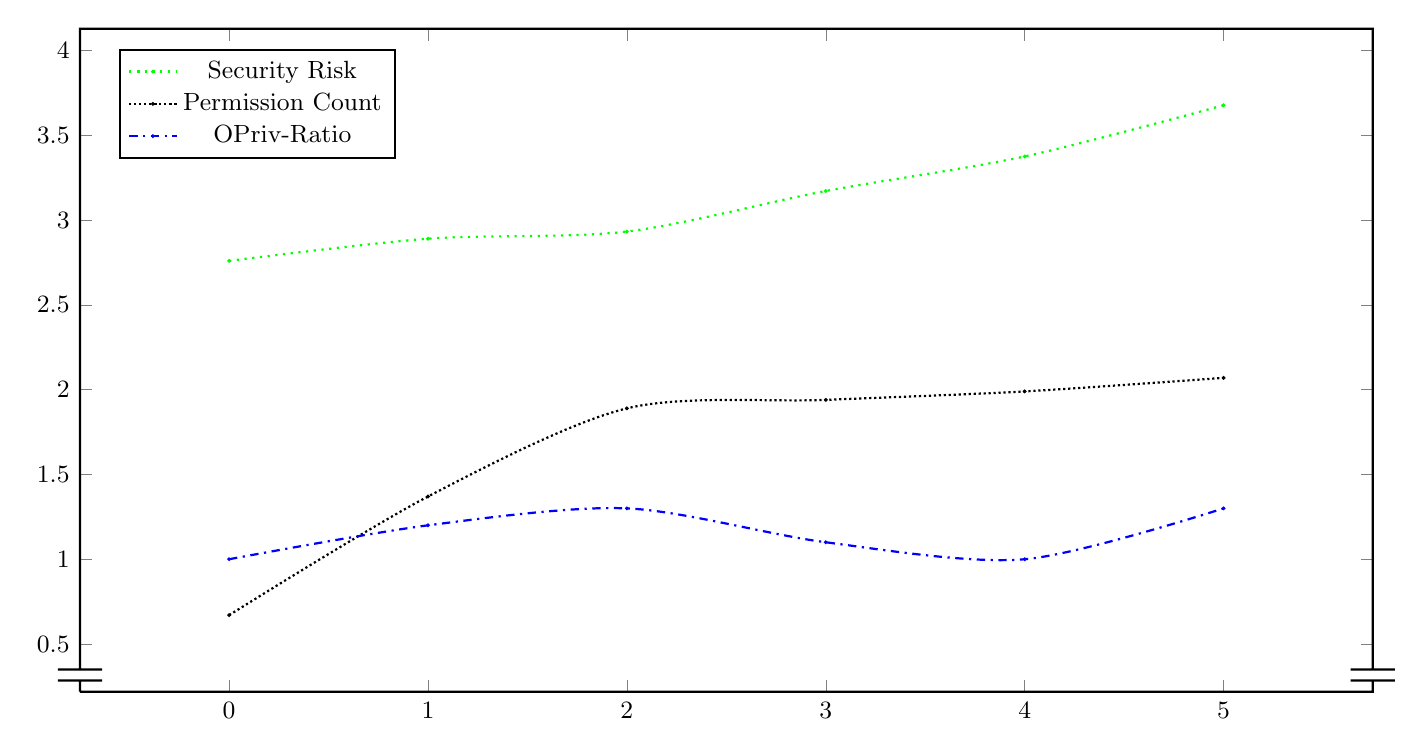
\begin{tikzpicture}
\begin{axis}[
   smooth,
   width=18cm,
   height=10cm,
   enlargelimits=0.15,
  %xlabel={Version Group \# (e.g. 0 is $0 \leq v < 1.0$)}
  ,
  %ylabel={Count},
  symbolic x coords={0,1,2,3,4,5,6,7},
  xtick=data,
  x tick label style={rotate=0,anchor=north},
% legend pos=north west, % original
  legend pos=north west, font=\small, ,line width=.8pt,mark size=.2pt,
 axis y discontinuity=parallel,
]


\addplot [color=green,dotted,mark=*,mark options={solid},smooth] plot coordinates {(0,2.76) (1,2.891) (2,2.933) (3,3.172) (4,3.376) (5,3.678)};
\addlegendentry{Security Risk}


\addplot [color=black,densely dotted,mark=*,mark options={solid},smooth] plot coordinates {(0,.67) (1,1.37) (2,1.89) (3,1.94) (4,1.99) (5,2.07)};
\addlegendentry{Permission Count}


\addplot [color=blue,dashdotted,mark=*,mark options={solid},smooth] plot coordinates {(0,1.0) (1,1.2) (2,1.3) (3,1.1) (4,1.0) (5,1.3)};
\addlegendentry{OPriv-Ratio}


\end{axis}
\end{tikzpicture}
\label{fig:VersionEffect}
\caption{Maturity and Metrics (RQX) - Needs to be updated}
\end{center}
\end{figure*}

%%% What are the most pervasive over privs and when did they occur?
\todo{Version\_order is not correct in the queries and needs to be fixed.}













\subsection{Overpriv Analysis}
\todo{Look at some specific apps here and do more of an in depth analysis}
In order to better understand why over privileges \& vulnerabilities occur in Android applications, we selected several open source Android apps from the F-Droid data set and analyzed their development process by examining both their Git histories, application version histories, and the source code of each app. We chose apps that were reasonably popular and.... We will discuss the X selected apps below

https://github.com/AndroSec/VersionControlExtractor.git



%%% Find the names of the overprivs for each version
%       See when each was added during the development cycle
%       Who added them
%       What was the commit message





\textbf{2048}\\
% 2048 -
%   http://androsec.rit.edu/analytics/280
%   http://darwin.rit.edu/analytics/159

%       No data for darwin, but Manifest info on Androsec

%2048\footnote{\url{https://play.google.com/store/apps/details?id=com.estoty.game2048}} is a popular Number puzzle game with over XXX downloads. F-Droid holds a popular port of the game


%   14 manifest commits
%   4 major versions
%   37 GH commits % Not many
%   No overprivs in any versions






%% Do people know they are making a commit that causes the over priv?


%% Who is making the over privs







%%% Next analyze some apps in the Androsec dataset
%%% Added 4/29
% In the analysis of GooglePlay apps, we found that Communication, productivity and social apps had the highest rate of overpriviledge. In order to better understand why these over privileges are occurring, we examined several applications from each genre from the F-Droid Android repository. We sought to determine when, why and how these over privileges were introduced.


%%%%% Probably not needed
% The first step was to find apps that existed in both data sets for each of the respective genres. This was somewhat difficult since both data sets do not contain the same apps, and the F-droid repository only contains XXX apps while our GooglePlay repo holds a much larger number of apps, XXX.



%%% Specific Apps

    %wifi automatic
    %FTP Server (Demo)

    %UberSync for Facebook
    %XBMC Remote
    %Document Viewer



%? Are the same categories the most overprived in both darwin & Androsec


%- Compare darwin vs Androsec genre rates
%- Examine some Androsec apps. Find good examples to examine.





% FBReader - 818
%   A commit message describes that the permission was added
%   Most versions of the app have no overprivs, until the very end.

% ACal - 442


% ownCloud - 528



% NetworkLog - 761


% Terminal Emulator - 710



% WordPress - 1158
%   Overpriv is added near the final version of the app
%       Camera was the overpriv
% No manifest commit info



%  --- Double check all of these to make sure that they actually have information


%%%% Some good basic examples of information changing
% --- Look at what I started to write up



%%% Look at the overall rate of permissions compared to the rate of overprivs
%%%%    Look @ recorded permissions either in the DB or in the Manifest files for all apps as an aggregate




% UberSync for Facebook 963/654
%   Manifest commits:       33
%   Major versions:         5
%   GH commits              129
%   Overprivs:              Oprivs increase over time



% XBMC Remote 144/638
%   Manifest commits:       X
%   Major versions:         X
%   GH commits              X
%   Overprivs:              X





% AppName X/X
%   Manifest commits:       X
%   Major versions:         X
%   GH commits              X
%   Overprivs:              X



%%% More case study items

% org.durka.hallmonitor
%







\section{Security \& User Ratings}
\label{sec: userratings}
% Use much of what we had for our rejected MSR paper





\section{Recommendations}
\label{sec:recommendations}







\section{Publicly Available Dataset}
\label{sec:dataset}

% Talk about Darwin and Androsec here
% Most of this can be reused from the ICSE paper
% Make sure this doesn't tie too much into what we are doing for SAC



\section{Limitations}
\label{sec:limitations}




\section{Related Work}
\label{sec: relatedwork}
%% External file so it can be easily included/excluded
%\vspace{-10pt}
\section{Related Work}
\label{sec: relatedwork}
While no previous works have investigated architectural tactics as we have, numerous previous studies have analyzed code clones and their impact on software development. Juergens et al.\cite{juergens2009code} studied the consequences that code clones had on program correctness. This work found that commercial and open source software systems often suffer from inconsistent changes due to the presence of code clones, thus leading to possible system faults and increased maintenance costs. Many previous works have stated that code clones are undesirable since they often lead to more bugs and make their remediation process more difficult and expensive~\cite{Mondal:2012:ESC:2387358.2387360,Duala-Ekoko:2010:CRD:1767751.1767754}. Other research has shown that clones may also substantially raise the maintenance costs associated with an application~\cite{juergens2009code}, the importance of which is highlighted by the fact that the maintenance phase of a project has been found to encompass between 40\% and 90\% of the total cost of a software project~\cite{Shukla:2008:ESM:1342211.1342232}. Ultimately, unintentionally making inconsistently applied bug fixes to cloned code across a software system increases the likeliness of further system faults~\cite{Deissenboeck_2010}.


%%% Mention some other clone detection techniques
Nicad is a powerful text-based hybrid clone detection technique, but there are numerous other popular clone detection tools and techniques. Some of which include Simian\footnote{\url{http://www.redhillconsulting.com.au/products/simian/}}, CloneDR\footnote{\url{http://www.semdesigns.com/products/clone/}}, MeCC\footnote{\url{http://ropas.snu.ac.kr/mecc/}}, CCCD~\cite{Krutz:2015:EEU:2695664.2695929}, and Simcad~\cite{6613857}. We are confident in our selection of Nicad due to its effectiveness which has been demonstrated in previous research~\cite{Roy:2008:NAD:1437898.1438600}. 




%% Why developers create code clones

%%% What has Nicad been used for in the past


%%% Code Reuse
Although code clones have been demonstrated to be detrimental in certain situations, code reuse is imperative for most software development projects. Numerous previous works have studied software reuse on both open source, and commercial applications. Code reuse has been found to save significant time and resources for most projects, along with increasing the overall quality of the software~\cite{493415}. Heinemann~\cite{Heinemann:2011:ENS:2022115.2022138} performed an empirical study in 20 open source projects and analyzed 3.3 MLOC. Their analysis found that 9 of the 20 examined applications had software reuse rates of over 50\%. Fortunately, most of the reuse was through black-box reuse, and not through simply copying \& pasting source code from the various applications. Mockus~\cite{mockus2007large} conducted a study to determine the extent of software reuse in open source projects, identify the most reused code, and investigate patterns of large-scale reuse. This work found that 50\% of the files were being used in more than one project, and that the most widely reused components were generally small, although some were comprised of hundreds of files.

Although there have been a few source code recommender systems~\cite{DBLP:conf/icse/McMillanHPCM12,6340250}, the primary focus of these works are on generic source code, and not tactical code snippets. Therefore the challenges of obtaining and recommending architecturally significant code is still unexplored. This paper conducted a qualitative study and reported challenges related to implementation and reuse of tactical code snippets.


 



%%%%%%%% 
% Make sure to point out what is new
% 	Really point out what our take home message is -- Make it an emph ?
% 






%%%%

%Nicad\cite{Roy:2008:NAD:1437898.1438600}: A text-based hybrid tool that combines the advantages of text and tree-based structural analysis. Clone identification and normalization are conducted using pretty printing and longest common subsequences. Nicad is compatible with C, Java, C#, and Python and has been found to have the ability to detect type-1, type- 2, and type-3 clones.



% Find papers that look at manifest files/permissions to see how they evolve over time





\section{Conclusion}
\label{sec: conclusion}


%\section*{Acknowledgment}

%This research would not have been possible without the hard work by two dedicated Software Engineering Students: Shannon Trudeau and Adam Blaine. We would like to thank them for their dedication and the insights they have provided on this project.


\balance
\bibliographystyle{abbrv} % This style looks to be good. Check out: http://cse.unl.edu/~tyu/docs/simrt.pdf
\bibliography{AndroidData}

% that's all folks

\end{document}


%%%%
%   ICSE = 10 pages



%%%% Actions
% When reporting information back, really try to examine the "WHYS" for everything. Do not just present results.
% ? Should we focus on Jlint and things at all?


%%% Todo
% Put into desired format & page length
% Keep consistent with over priv/over permission - See what was said in MSR paper that did not get in
% How can Darwin be tied into this somehow


%%% Other possible RQs
%   Do more different committers lead to worse code?
%   Look at general quality of commit messages



% Get apps with at least X versions from Darwin?
%   May not have enough of a time period between each app for them to be useful


% Really focus on why they occur
% Tie user ratings into this paper. ICSE?
%


% ? - Related paper to see if permissions are being removed
%   WHY are they being added/removed
%   % Check to see if specific function calls are over/underprived -
%


% Will really need to dig deep and say WHY


% Write in a way that is clear. Really drive home what you are doing. Readers make the decision in the 1st page if they are going to accept/reject the paper.

% Try downloading older versions of apps - http://www.apk4fun.com/apk/6152/


% ICSE - 10 pages 